
\documentclass[10pt, conference]{IEEEtran}

\usepackage{algorithmic}
\usepackage{amsmath}
\usepackage{amssymb}
\usepackage{amsthm}
\usepackage{balance}
\usepackage{cite}
\usepackage{color}
\usepackage{graphicx}
\usepackage{gregmath}
\usepackage{framed}
\usepackage{stmaryrd}
\usepackage{subfigure}
\usepackage{times}
\usepackage{url}

\graphicspath{{./pdf/}}
\pdfoutput=1

\pagestyle{empty}

%-------------------------------------------------------------------------
\begin{document}


\title{\ \\ \bf \Large  A Study of an Incremental Spectral Meta-Learner for Nonstationary Environments}   
\author{\IEEEauthorblockN{Gregory Ditzler 
  \thanks{Gregory Ditzler is with the Department of Electrical 
    \& Computer Engineering at the University of Arizona, Tucson, AZ.
     }
   \thanks{Author email: ditzler@email.arizona.edu}
  }
}
\IEEEoverridecommandlockouts
\maketitle



%-------------------------------------------------------------------------
\begin{abstract}

Incrementally learning from large volumes of streaming data over time is a problem that is of crucial importance to the computational intelligence community, especially in scenarios where it is impractical or simply unfeasible to store all historical data.  Learning  becomes a particularly challenging problem when the probabilistic properties of the data are changing with time (i.e., gradual, abrupt, etc.), and there is scarce availability of class labels.  Many existing strategies for learning in nonstationary environments use the most recent batch of training data to tune their parameters (e.g., calculate classifier voting weights), and never reassess these parameters when the unlabeled test data arrive.  Making a limited drift assumption is generally one way to justify not needing to re-evaluate the parameters of a classifiers; however, labeled data that  have already been learned if presented to the classifier for testing could be forgotten because the data was not observed for a long time. This is one form of abrupt concept drift with unlabeled data.  In this work, an incremental spectral learning meta-classifier is presented for learning in nonstationary environments such that: (i) new classifiers can be added into an ensemble when labeled data are available, (ii) the ensemble voting weights are determined from the unlabeled test data to boost recollection of previously learned distributions of data,  and (iii) the limited drift assumption is removed from the test-then-train evaluation paradigm. We benchmark our proposed approach on several widely used concept drift data sets. 


\end{abstract}

%-------------------------------------------------------------------------
\section{Introduction}
\label{sec:mot}

The traditional supervised machine learning paradigm assumes that the training and testing data are sampled from a fixed -- albeit unknown -- probability distribution; however, this assumption are often incorrect and if violated could result in an inaccurate classifier. 
In the setting of learning in nonstationary environments,  data arrive at a fast rate from a stream. The data  are presented for learning  either in batches (incremental) or a single instance at a time (online). 
For the purposes of this research we shall strictly focus on the batch scenario. At each time $t$ a new batch of data are presented; however, in the case of nonstationary environments, the batches of data across  time points are {\em not} assumed to be sampled i.i.d. from a fixed distribution $\Dcal$. 
Hence algorithms designed to learn in a nonstationary environment must be capable of learning from new data, while learning to forget old or irrelevant knowledge. This problem of learning and forgetting is widely known as the {\em stability-plasticity dilemma} \cite{Grossberg1988NN}. 


\begin{figure}
\centering
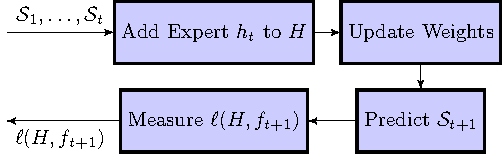
\includegraphics[width=.5\textwidth]{survey-f1.pdf}
\caption{High-level block diagram used by incremental learning ensembles in nonstationary environments. Data are received in batches $\Scal_t$ over time. A classifier $h_t$ is built with the new data, which is then added to the ensemble $H$. Unlabeled data from $\Scal_{t+1}$ is classified using the ensemble $H$ and a loss, $\ell(\cdot,\cdot)$, is measured when labels from $\Scal_{t+1}$ arrive \cite{Ditzler2015CIM}. }
\label{fig:learning}
\end{figure}


Multiple classifier systems are quite popular in the nonstationary environments community because of their ability to strike a balance between stability and plasticity \cite{Ditzler2013TKDE, Minku2012TKDE, Kuncheva2004MCS}. 
Stability and plasticity can be controlled with a multiple classifier system by adding and removing classifiers, respectively. The classifiers in the ensemble are assigned a  voting weight. 
The weight of the classifier can be used to determine those classifiers that are the most relevant at some time $t$, where the weights are typically determined by the error on the most recent training data, and new classifiers can be added to the ensemble to incorporate new knowledge (see Figure \ref{fig:learning}). However, we observe a potential flaw with the classifier weighting strategy, which is that the data time $t$ and $t+1$ must be ``similar'' for this technique to work and it does not take into account the possibility that the target concept may have already been learned. This is in essence what is referred to as the limited drift assumption in latency verification problems \cite{Souza2015ICDM, Dyer2014TNNLS, Sarnelle2015IJCNN}. 
An ensemble would be expected to perform poorly if the nonstationary environment were to encounter an abrupt change back to an old environment (i.e., reoccurring concept that is suddenly reintroduced \cite{Alippi2013TNNLS, Elwell2011TNN}). 
Furthermore, learning to forget old knowledge could potentially implement a form of catastrophic forgetting, which not ideal and does not follow the prescription of how we as humans learn. 

To illustrate this area of opportunity within learning in nonstationary environments, consider the learning scenario  in Figure \ref{fig:concepts}. It is assumed that data are not stored after  they are learned (i.e., the incremental learning assumption \cite{Bifet2009KDD, Polikar2001TSMC}). First, many of the state-of-the-art algorithms for learning in nonstationary environments track the drifting environments and score the quality of a classifier based upon the most recent training data \cite{Ditzler2013TKDE, Dyer2014TNNLS, Alippi2008TNNb, Bifet2009KDD, Nishida2007MLC}. 
In Figure \ref{fig:concepts}, a stream of data contains four concepts at five time points. The concept can be thought of as a probability distribution, $\Dcal_t$, that is specific to time $t$. The concepts gradually change in the training (i.e., labeled data), and testing (i.e., unlabeled data) streams until $t_5$, which {concept 1} appears in the testing stream even though this concept has not been presented ``recently''.  
The nonstationary learning literature has examined recalling reoccurring concepts \cite{Alippi2013TNNLS}; however, identifying the concept from unlabeled data still remains a challenging problem if old data are not retained. 


One of the central issues becomes detecting that the test data presented at a time, is an old concept (distribution) that was learned in the past. This is a non-trivial problem because it is assumed that the algorithms no longer have access to the old data. A divergence metric could be used to measure the discrepancies between the two distributions of the data if labeled data were available from the history; however, this would violate the incremental learning assumption \cite{Polikar2001TSMC}. 
Therefore, we present an incremental learning framework based on advances in spectral learning to adapt the weights of a classifier without access to labeled data, where the weights are proportional the error on the unlabeled data. 


\begin{figure}
\centering
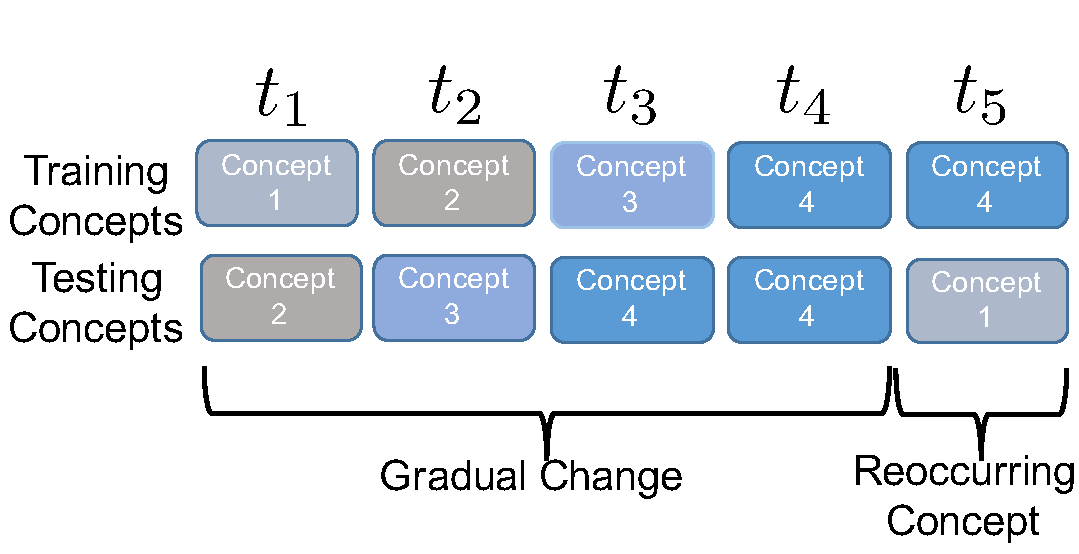
\includegraphics[width=.48\textwidth]{concepts.pdf}
\caption{A illustration of a nonstationary environment where concepts are being learning over time. Concepts can be interpreted as {concept 1} is closer to {concept 2} than it is to {concept 3}. Thus an ensemble algorithm could perform poorly when {concept 1} is re-introduced in the testing sequence, because the ensemble weights were determined from {concept 4} at $t=5$. }
\label{fig:concepts}
\end{figure}


The rest of this manuscript is organized as follows:  Section \ref{sec:rwork} presents related work,  Section \ref{sec:proposed} presents an  algorithm for learning in the presence of a nonstationary environment,  Section \ref{sec:exp} evaluates the proposed approach on real-world data streams, and Section \ref{sec:conc} draws conclusions and future work.

%-------------------------------------------------------------------------
\section{Related Works}
\label{sec:rwork}

Supervised learning in  nonstationary environments is becoming a mature field; however, leveraging unlabeled data to identify the concept or adjust algorithm parameters still remains a challenging problem. This section highlights related work in nonstationary environments and areas that are closely related. 


\subsection{Multiple Classifier Systems}
As mentioned earlier, multiple classifier systems have been quite popular in the NSE community due their ability to strike a balance between stability and plasticity \cite{Ditzler2013TKDE, Minku2012TKDE, Kuncheva2004MCS}. The weight of the classifier can be used to determine the classifiers that are the most relevant at some time $t$, where the weights are typically determined using an error measurement on the most recent training data (see Figure \ref{fig:learning}).  
It is unlikely that the ensemble will be able to identify the best classifier to predict on the data at time $t+1$ without access to some labeled data from the test data set. 
This idea was motivated in the end of Section \ref{sec:mot}, and Gao et al. showed that if the testing data are sampled from an unknown distribution (i.e., one of the $t$ distributions observed until time $t$) that uniform weights are the best strategy \cite{Gao2007IEEEICDM, Gao2007SIAMICDM, Gao2008IC}. 
In the case of limited drift, the most recent training data are used to re-adjust the classifier weights \cite{Ditzler2013TKDE, Elwell2011TNN, Tsymbal2008IF}. Thus, the weights of the classifiers should be re-adjusted based off of the most recent test data to attempt to identify the classifiers that will perform better than the other on the most recent (unlabeled) test data. 

Recent work has come out of the transfer learning community to ameliorate the effect of identify the most accurate predictions \cite{Ruvolo2013ICML}; however, the task may need to be known {\em a priori}, which can be difficult assume this piece of information would be known. To work around the issue of knowing the task, an active task selection approach was developed \cite{Ruvolo2013AAAI, Ammar2015ICML}. Though the approaches mentioned thus far primarily fit into a solely supervised view of learning in a nonstationary environment. 

\subsection{Extreme Verification Latency}
There have been several efforts to incorporate unlabeled data into the models via semi-supervised or transductive \cite{Ditzler2011IJCNN, Ditzler2012WCCI}, and algorithms that handle extreme verification latency \cite{Souza2015ICDM, Dyer2014TNNLS, Dyer2012IJCNN, Capo2013IJCNN, Sarnelle2015IJCNN, Krempl2011ICDMW, Krempl2011AIDA}.  Extreme verification latency (ELV) assumes that an initial batch of labeled data are presented for building a classifier then the entire data stream is unlabeled and assumed to be nonstationary. The fundamental assumption of ELV is that the drift must be incremental in nature \cite{Sarnelle2015IJCNN, Souza2015ICDM}, which prohibits old concepts from being abruptly introduced. Our learning setting removes this assumption to the point where if new labeled data are available to build a classifier then a classifier can be learned; however, the mechanism in which the prediction happens is different than of ELV. 
With the exception of a few works, such as that of Zhang et al. \cite{Zhang2010ICDM}, which combines classification and clustering, taking advantage of unlabeled data has not been fully exploited within concept drift literature, and other similar approaches can be found in the consensus maximization literature \cite{Dong2014ICDM, Gao2012TKDE, Gao2009NIPS}; however, these approaches have yet to be evaluated in a nonstationary environment.



\subsection{Spectral Meta-Learning}

All of the approaches so far (regardless of considering unlabeled data) fix the classifier's weight in the ensemble  vote. More specifically, if an ensemble provides a prediction $H(\x) = \sum_i \alpha_i\,h_i(\x)$ (where $h_i(\x) \in \Rbb$ and $\alpha_i \in \Rbb_{+}$ are the $i$th classifier and classifier weight, respectively), the weights remain fixed regardless of $\xbf$. 
A prediction using the weighted vote will not be effective if data are sampled from the probability distribution that is different than the one used to produce $\alpha_i$. If a subset of predictors are better at predicting on $\xbf$ because of the domain they were learned, then we would want them to have a higher weight. This type of weight adjustment strategy has been proven to be successful for classifiers that are trained on very different classes \cite{Ditzler2013IJCNN, Muhlbaier2009TNN}. 

Our proposed research examines the use of spectral-meta learner (SML), which was recently proposed by Parisi et al. \cite{Parisi2014PNAS}, to dynamically assign the classifier's weight when new data become available. In Parisi et al.'s work, they present spectral-based approach that estimates the (balanced) error of a classifier from unlabeled data that is sampled i.i.d. from a distribution $\Dcal$, where the balanced error is the average of the recall for each class. 
The authors of \cite{Parisi2014PNAS} show that a matrix  
\begin{align}
\Cbf_{ij} := \Ebb[(h_j(\xbf)-\Ebb[h_i(\xbf)])(h_j(\xbf)-\Ebb[h_i(\xbf)]) ] \nonumber
\end{align} 
\noindent has  off diagonal entries that are equal to a rank-one matrix $\Rbf = \lambda \vbf\vbf^\T$, where $\vbf$ is an eigenvector whose entries are proportional to the balanced accuracies of the classifiers, where $i,j \in [t]$. 




%-------------------------------------------------------------------------
\section{An Incremental SML Framework}
\label{sec:proposed}

The following section describes an SML approach for learning in a nonstationary environment, such that the environment can be tracked and recurring concepts can be addressed without being provided labeled data.  

%-------------------------------------------------------------------------
\subsection{Algorithm Description}

The pseudo-code for the proposed approach can be found in Figure \ref{alg:transe}. We refer to this algorithm as {\em S}pectral {\em E}nsemble for {\em N}on{\em S}tationary {\em E}nvironments (Sense). Sense is an incremental version of  Parisi et al.'s SML approach, whose goal  is to build up a knowledge base of classifiers when labeled data ($\Acal_t$) are available at time $t$ and efficiently predict on the unlabeled data ($\Bcal_t$) by dynamically adjusting the classifier voting weights. The data $\Acal_t$ and $\Bcal_t$ are assumed to be sampled two fixed probability distributions (e.g., the data stream could be similar to the learning scenario presented in Figure \ref{fig:concepts}).

\begin{figure}
  \centering
  \begin{framed}\small
    \begin{algorithmic}[1]
      \INPUT labeled data $\Acal_t=\{\left(\xbf_i,y_i\right)\}_{i=1}^{m_t}$,
        unlabeled test data $\Bcal_t=\{\left(\xbf_j\right)\}_{j=1}^{n_t}$, and 
        {\sc Learn} base classification algorithm
      \vspace{1em}
	  \FOR{$t=1,2,\ldots$}
	    \STATE Call {\sc Learn} with $\Acal_t$ and receive classifier  $h_t$
        \STATE Predict class labels for $\xbf_j\in\Bcal_t$ to construct $\Hbf_t \in \Rbb^{t \times n_t}$
        \STATE $\Cbf_t = \textrm{cov}(\Hbf_t)$
        \STATE Using $\Cbf_t$  compute the adjusted diagonal entries in $\Rbf_t$ (see \cite{Parisi2014PNAS} for details)
        \STATE $\Vbf_t,\lambda_t = \textrm{eig}(\Rbf_t)$
        \STATE Calculate class labels 
          \begin{equation}
            \label{eq:weight votes}
            \fbf_t = \textrm{sign}\left(\Hbf_t^\T\Vbf_{t,1}\right)
          \end{equation}
          where $\Vbf_{t,1}$ is the leading eigenvector. 
	  \ENDFOR
	  \OUTPUT Prediction's $\fbf_t$ at each time $t$.
    \end{algorithmic}
  \end{framed}
  \caption{{\em S}pectral {\em E}nsemble {\em N}on{\em S}tationary {\em E}nvironments (SENSE)}
  \label{alg:transe}
\end{figure}

{\bf\noindent Learning Base Models and Diversity}\\
The Sense algorithm begins by generating a classifier, $h_t$, using an algorithm \textsc{Learn} on the labeled data (see line 2 in Figure \ref{alg:transe}). \textsc{Learn} could be any classification algorithm such as logistic regression, decision trees or support vector machines. This classifier is meant to act as a model for the data that was received at time $t$, which allows Sense to discard $\Acal_t$ after the classifier is learned, thus making the algorithm adhere to the definition of incremental learning \cite{Polikar2001TSMC}. It is important to observe this property of Sense because the data stream could be massive in the cardinality of observations and retaining such data could be computationally burdensome. The   {\em plasticity} of the ensemble is then increased by adding new classifiers into the ensemble when new data are available, and  labeled data are not required at each time step (though it is not shown in the pseudo code for simplicity). 

The classifiers $h_i$ for $i\in[t]:=\{1,\ldots,t\}$ will have diversity in their predictions simply because they were trained on different data sets (or concepts). Diversity within an ensemble has been shown to be beneficial to the ensemble's classification accuracy \cite{Kuncheva2004Book}, and Minku et al. showed that diversity is particularly beneficial for in nonstationary environments.  
To increase the diversity within the ensemble of classifiers, \textsc{Learn} can be varied at each time step between a finite selection of choice classifiers. For this work, the diversity is solely controlled by the drifting probability distributions. 
\vspace{.5em}

{\bf\noindent Error Estimation}\\
The ensemble of classifiers retains the information about the concept within classifier. Given some unlabeled data $\xbf \in \Bcal_t$ (see line 3 in Figure \ref{alg:transe}), the ensemble decision is given by 
\begin{align}
H(\x) = \textrm{sign}\left(\sum_{i=1}^{t} \alpha_i\,h_i(\x)\right)
\end{align}
\noindent which is a weighted majority vote with weights $\alpha_i \in \Rbb_{+}$ and $h_i(\x) \in \Rbb$. Unfortunately, as stated earlier,  determining an optimal choice of $\alpha_i$ is very difficult in practice if labeled data from the test data are not available.  To get around this unknown, the vast majority of nonstationary learning algorithms make a limited drift assumption. If the assumption were true then setting $\alpha_i$ inversely proportional to the error on $\Acal_t$, which is given by 
\begin{align}
\alpha_i = \log\left(\frac{1 - \widehat{\epsilon}_i}{\widehat{\epsilon}_i}\right), \nonumber
\end{align}
would be sufficient (where $\widehat{\epsilon}_i$ is the estimate error). However, if this assumption were not true (see Figure \ref{fig:concepts}) then the weighted majority strategy is almost surely going to fail. 


Parisi et al.'s spectral meta-learning (SML) algorithm provides an decision-theoretic approach to estimating the error of a classifier on unlabeled data \cite{Parisi2014PNAS}. 
To perform SML's error estimation, the individual classifiers ($h_i(\xbf_j)\in\{\pm1\}$) predict class labels for $\xbf_j\in\Bcal_t$ to construct a matrix $\Hbf_t \in \Rbb^{t \times n_t}$ that contains the predictions by each classifier in the ensemble on each sample in $\Bcal_t$ (see line 3 in Figure \ref{alg:transe}). The off-diagonals of the covariance ($\Cbf_t$) for $\Hbf_t$ are identical to those of a rank-one matrix, whose eigenvalues ($\Vbf_t \in\Rbb^{t \times 1}$) are proportional to the balanced accuracies of the $t$ classifiers (see lines 5 \& 6 in Figure \ref{alg:transe}). The weights are used directly for voting. 

The proposed algorithm thus implements an incremental learning approach with SML to learn in a nonstationary environment. One of the key distinctions between the learning process of traditional SML and Sense is that SML used different classifiers trained on a static distribution, whereas we are considering a nonstationary setting. 


%-------------------------------------------------------------------------
\section{Experiments}
\label{sec:exp}

To demonstrate the efficacy of the SML strategy for incremental learning in nonstationary environments, we evaluated the approach on several data streams that have become standard benchmarks.  
The experiments were run on on a machine with four Intel Xeon E7-4830 and 256GB of RAM. 



%-------------------------------------------------------------------------
\subsection{Evaluation Statistics, Benchmark Algorithms and Data Sets}


The proposed algorithm was benchmarked against several real-world and synthetic data sets. Furthermore, we examined the performance in terms of the raw classification error and the $\kappa$-statistic. The raw classification error is the number of missed classifications over the total number of instances classified (i.e., standard classification error). 

The $\kappa$-statistic is a measurement of the agreement between two classifier who each classify $N$ instances into $C$ classes \cite{Galton1982Kappa}. More formally this is calculated as
\begin{align}
  \kappa = \frac{p_0 - p_e}{1 - p_e}
\end{align}
where $p_0$ is the relative observed agreement among, and $p_e$ the probability that a chance classifier makes a correct prediction. One of the advantages of the $\kappa$-statistic is that is captures the balanced classification accuracy (i.e., performs well against all class, not just a majority class). 

\begin{figure*}
\centering
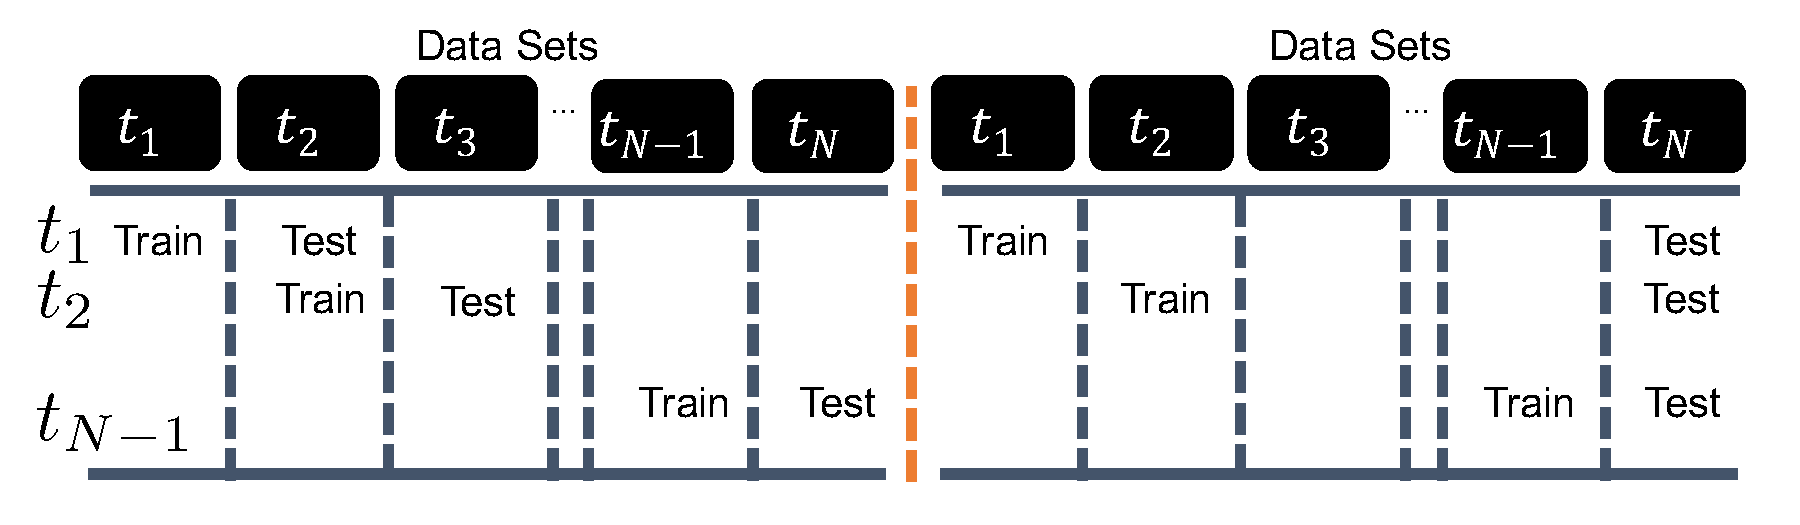
\includegraphics[width=\textwidth]{procedure.pdf}
\caption{Two evaluation schemes for evaluating classifiers on their ability to recall and learn new knowledge (schemes are separated by the dashed orange bar in the center of the figure). The evaluation scheme on the left, also known as a test-then-train setting, examines a classifiers ability to track a nonstationary environment by training in data at time $t_{N-1}$ and testing on $t_N$. The evaluation scheme on the right tests the ability of a classifier to learn from changing data streams over time, and be able to learn data at time $t_N$.}\label{fig:procedure.pdf}
\end{figure*}


\begin{table}
\caption{Properties of the data sets used for benchmarking. $\omega_1$ and $\omega_2$ are the percentages of each class.}\label{tab:data}
\begin{center}
\begin{tabular}{|l || c c c c |}
\hline
 & Samples & Features & $\omega_1$\% & $\omega_2$\% \\
\hline
\hline
poker & 805,384 & 10 & 51.6 & 48.4\\
noaa & 18,159 & 8 & 68.6 & 31.4\\
elec2 & 27,549 & 5 & 58.5  & 41.5\\
spam & 4,601 & 57 & 60.6  &39.4 \\
sea & 50,000 & 3 & 63.6 & 36.4\\
air & 539,383 & 7 & 55.5 & 44.5\\
\hline
\end{tabular}
\end{center}
\end{table}

Sense is benchmarked against three other data stream classification approaches: follow-the-leader (FTL), output averaging (AVG) and Learn\++.NSE (NSE). FTL measures the error on the most recent batch of labeled data and uses this classifier to make predictions on the next batch of unlabeled data. AVG averages the predictions of all of the classifiers in the ensemble, and Learn\++.NSE is an algorithm for learning in nonstationary environments that uses a time adjusted error function for dynamically re-weighting classifier. However, Learn\++.NSE still relies on the most recent labeled data to compute the voting weights and does not consider unlabeled data. 
CART was used as the base-classifier for all of the algorithms. 



\begin{table}[p]
\caption{Error averaged over all time points in each of the experiments. The number in parenthesis represents the rank on the algorithm on a data sets (lower is better). Errors are measured in the test-then-train scenario.}\label{tab:err-ttt}
\begin{center}
\begin{tabular}{|l || c c c c |}
\hline
& \bf Sense &\bf AVG &\bf NSE &\bf FTL \\
\hline
\hline
poker & 20.16 (3) & 22.23 (4) & 17.99 (2) & 16.91 (1) \\ 
noaa & 27.30 (3) & 24.11 (1) & 24.65 (2) & 36.91 (4) \\ 
elec2 & 35.27 (3) & 35.23 (2) & 31.57 (1) & 36.88 (4) \\ 
spam & 9.54 (1) & 9.84 (2) & 12.15 (3) & 20.51 (4) \\ 
sea & 6.62 (2) & 6.72 (3) & 3.76 (1) & 7.33 (4) \\ 
air & 37.42 (3) & 37.11 (2) & 36.07 (1) & 42.68 (4) \\ 
\hline
\hline
final & 2.5 & 2.33 & 1.67 & 3.5 \\ 
\hline
\end{tabular}
\end{center}
\end{table}

\begin{table}[p]
\caption{$\kappa$-statistic averaged over all time points in each of the experiments. $\kappa$-statistics are measured in the test-then-train scenario.}\label{tab:kap-ttt}
\begin{center}
\begin{tabular}{|l || c c c c |}
\hline
& \bf Sense &\bf AVG &\bf NSE &\bf FTL \\
\hline
\hline
poker & 60.08 (1) & 55.30 (4) & 59.73 (2) & 57.61 (3) \\ 
noaa & 36.03 (1) & 35.93 (2) & 35.83 (3) & 17.80 (4) \\ 
elec2 & 28.83 (2) & 23.13 (3) & 30.23 (1) & 21.76 (4) \\ 
spam & 79.51 (1) & 78.66 (2) & 73.98 (3) & 56.58 (4) \\ 
sea & 85.61 (2) & 85.38 (3) & 91.73 (1) & 83.75 (4) \\ 
air & 20.06 (1) & 18.91 (3) & 19.71 (2) & 9.54 (4) \\ 
\hline
\hline
final & 1.33 & 2.83 & 2.00 & 3.83 \\ 
\hline
\end{tabular}
\end{center}
\end{table}


\begin{table}[p]
\caption{Error averaged over all time points in each of the experiments.  Errors are measured in the test-on-hold-out scenario.}
\begin{center}
\begin{tabular}{|l || c  c c c |}
\hline
& \bf Sense &\bf AVG &\bf NSE &\bf FTL \\
\hline
\hline
poker & 16.34 (2) & 16.43 (3) & 15.29 (1) & 19.05 (4) \\ 
noaa & 44.58 (1) & 46.61 (2) & 47.14 (3) & 50.60 (4) \\ 
elec2 & 18.08 (1) & 23.14 (2) & 29.99 (3) & 40.32 (4) \\ 
spam & 9.00 (1) & 9.28 (2) & 10.84 (3) & 18.84 (4) \\ 
sea & 9.50 (2) & 9.85 (3) & 8.79 (1) & 10.78 (4) \\ 
air & 42.12 (1) & 44.23 (3) & 42.47 (2) & 46.73 (4) \\ 
\hline
\hline
 & 1.3333 & 2.5 & 2.1667 & 4 \\ 
\hline
\end{tabular}
\end{center}
\end{table}

\begin{table}[p]
\caption{$\kappa$-statistic averaged over all time points in each of the experiments. $\kappa$-statistics are measured in the test-on-hold-out scenario.}
\begin{center}
\begin{tabular}{|l || c c c c |}
\hline
& \bf Sense &\bf AVG &\bf NSE &\bf FTL \\
\hline
\hline
poker & 67.72 (2) & 67.48 (3) & 69.00 (1) & 59.80 (4) \\ 
noaa & 12.34 (3) & 15.82 (1) & 14.140 (2) & 5.18 (4) \\ 
elec2 & 63.82 (1) & 54.69 (2) & 42.18 (3) & 20.91 (4) \\ 
spam & 78.93 (1) & 77.94 (2) & 74.60 (3) & 57.10 (4) \\ 
sea & 80.07 (2) & 79.32 (3) & 81.52 (1) & 77.37 (4) \\ 
air & 21.40 (1) & 18.43 (3) & 19.27 (2) & 7.48 (4) \\ 
\hline
\hline
 & 1.6667 & 2.3333 & 2 & 4 \\ 
\hline
\end{tabular}
\end{center}
\end{table}

\begin{figure}
\centering
\subfigure[test-then-train]{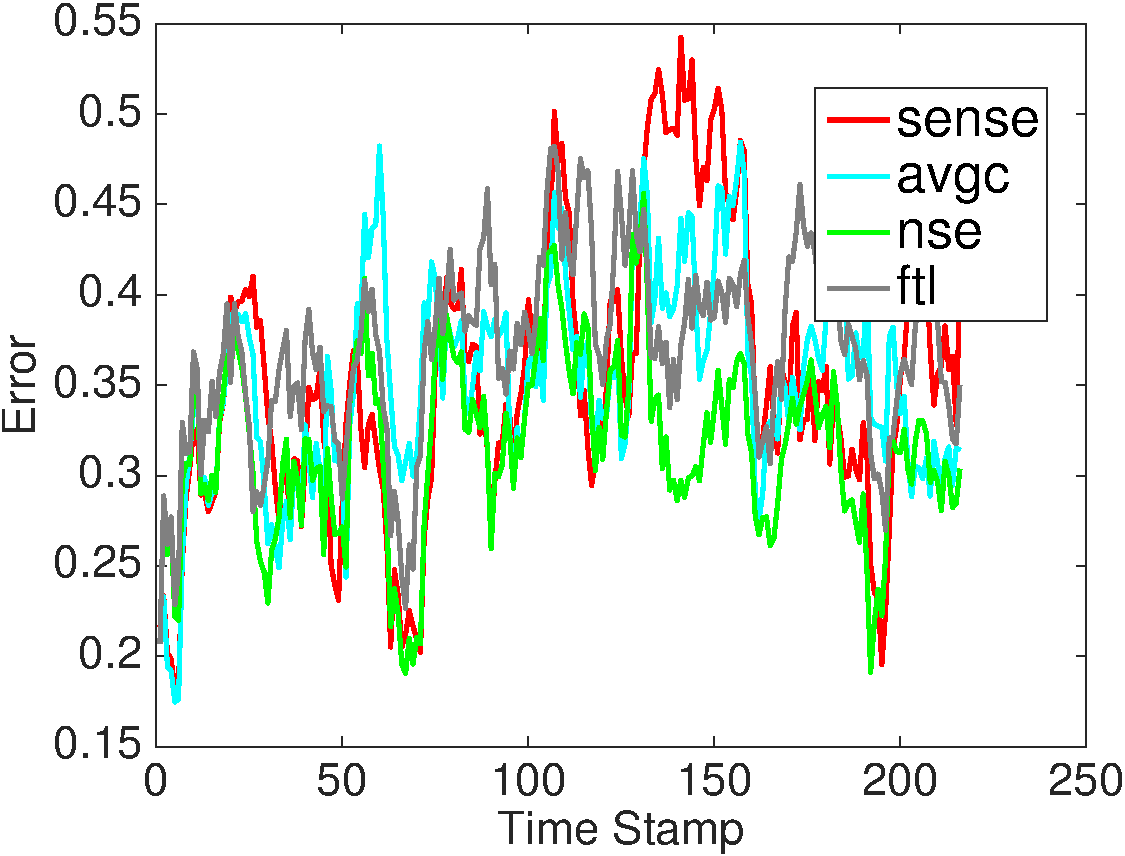
\includegraphics[width=.22\textwidth]{elec2_error.pdf}}
\subfigure[incremental]{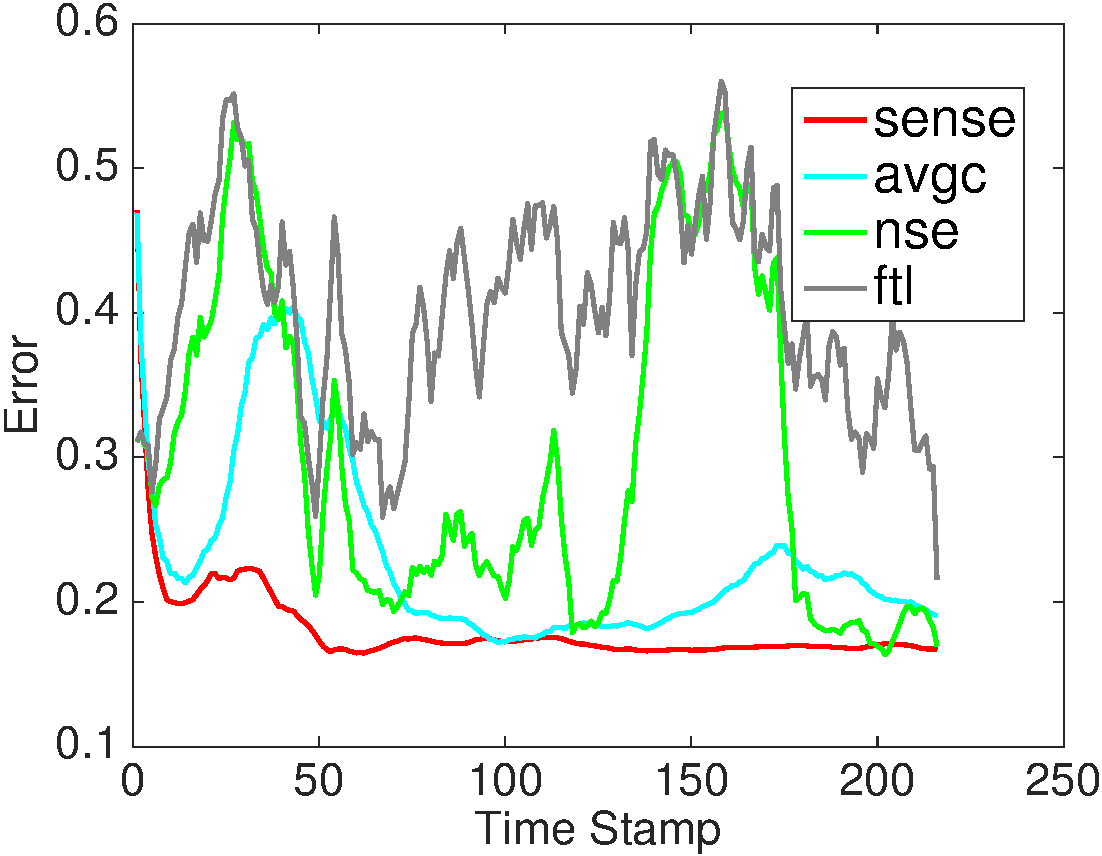
\includegraphics[width=.22\textwidth]{elec2_END_error.pdf}}
\caption{Classification error of the benchmarked algorithms on the elec2 data set.}
\end{figure}

\begin{figure}[h]
\centering
\subfigure[test-then-train]{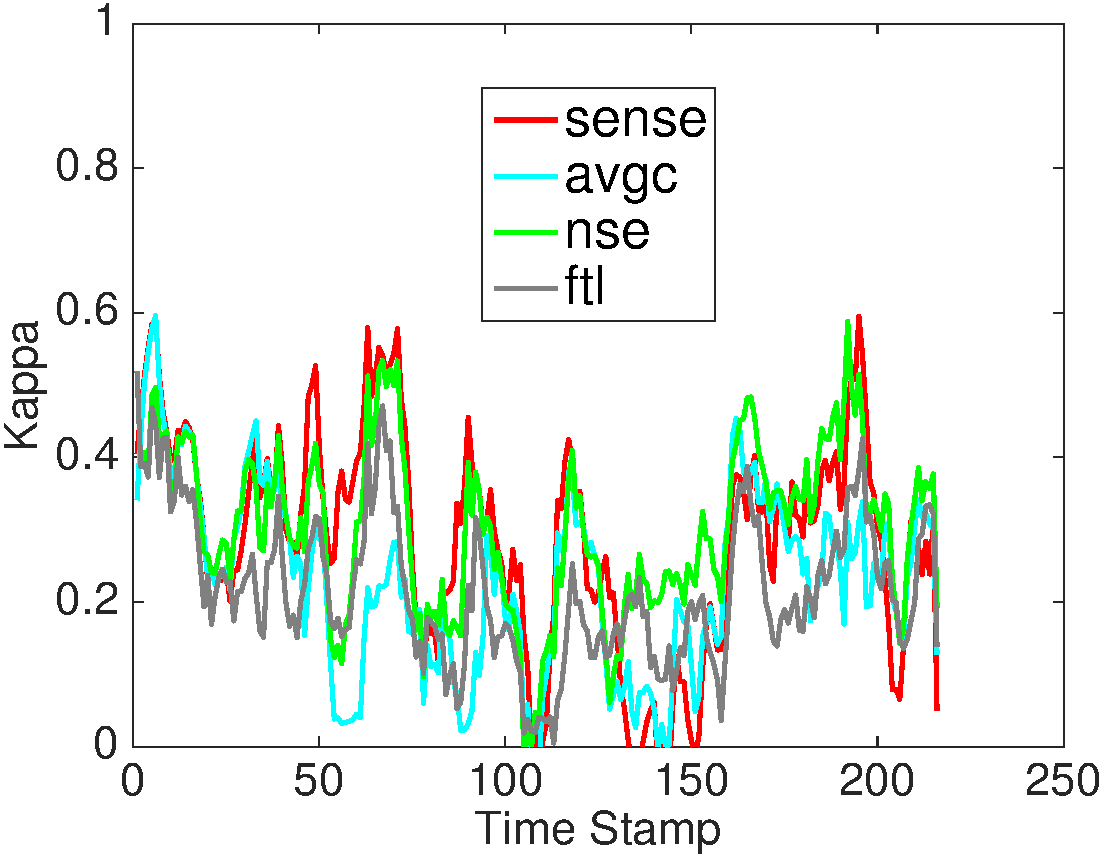
\includegraphics[width=.22\textwidth]{elec2_kappa.pdf}}
\subfigure[incremental]{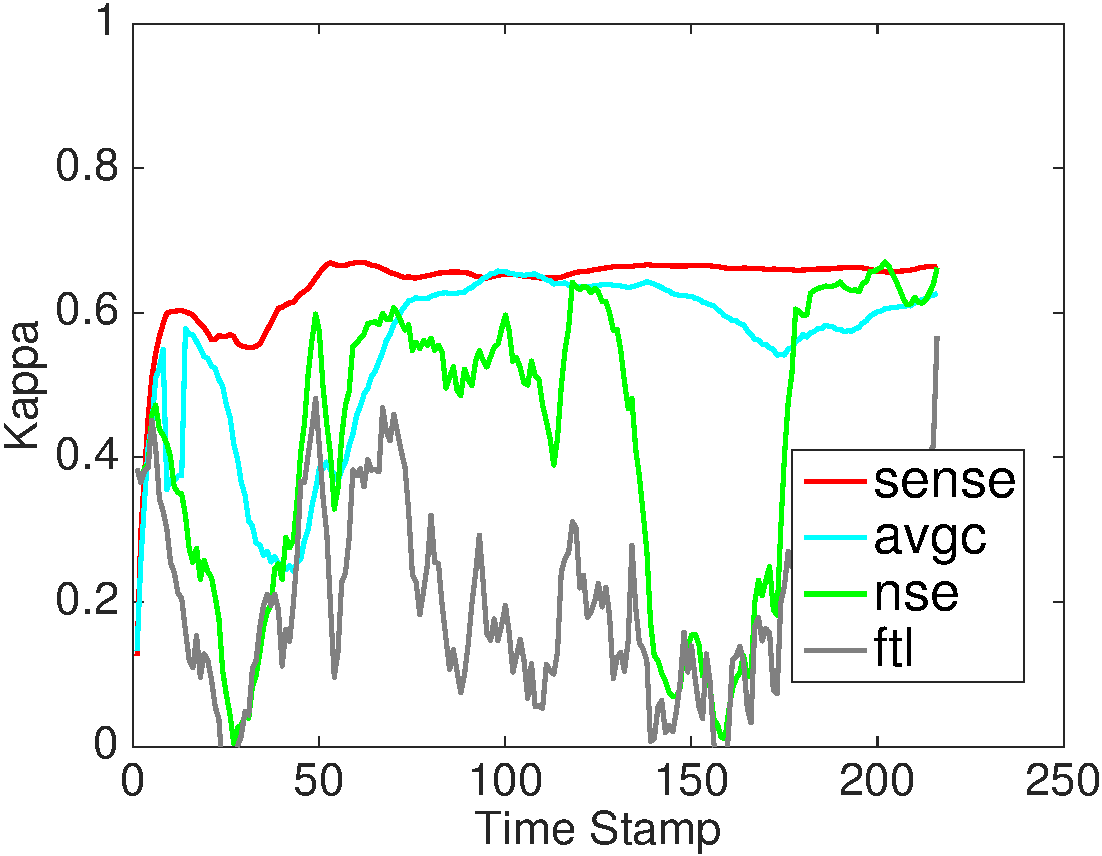
\includegraphics[width=.22\textwidth]{elec2_END_kappa.pdf}}
\caption{Classification kappa error of the benchmarked algorithms on the elec2 data set.}
\end{figure}




The data streams that were used as benchmarks are summarized below: 
\begin{itemize}
\item {\em Airlines} \cite{Ikonomovska2012Phd}: This data set contains flight arrival and departure details for commercial flights between October 1987 to April 2008. The objective is to predict if a flight will be delayed. We generated a data stream for using -- approximately -- the first 540k instances. 
\item {\em Electricity Pricing} \cite{Harries1999TR}: This data set provides time and demand fluctuations in the price of electricity in New South Wales, Australia.  The task is to predict whether the NSW price will be higher or lower than VICs in a 24-hour period.
\item {\em Poker Hand} \cite{Frank2010UCI}: The poker data contains poker cards and the objective is to predict the hand. This data set is converted to a binary classification problem such that the classes are approximately balanced. This particular data set represents a data stream classification problem that does not contain explicit concept drift. 
\item {\em SEA} \cite{Street2001KDD}: SEA is a synthetic data set with three feature where only two are relevant. This problem reduces to linear classification problem with abrupt changes in the hyperplane every 50 time steps. 
\item {\em Spam}: The spam data contains a collection of emails that are either spam or ham. 
\item {\em NOAA Weather} \cite{Elwell2011TNN}: This data set contains 50 years worth of data, which can provide not only cyclical seasonal changes, but also possibly long-term climate change. Daily measurements were taken for a variety of features such as temperature, pressure, visibility and wind speed, and the objective is to predict if it rained. 
\end{itemize}

A summary of the data stream properties can be found in Table \ref{tab:data}.






%-------------------------------------------------------------------------
\subsection{Evaluation Strategy}



The algorithms were evaluated using two different strategies (see Figure \ref{fig:procedure.pdf}). The strategy on the left is a standard test-then-train evaluation strategy, where data are used for testing (unlabeled data) prior to training on it (once the labels are received). This strategy is the most common form of evaluation for data streams. However, the test-then-train strategy is not ideal for the data streams if we want to evaluate the learning scenario presented in Figure \ref{fig:concepts}. To evaluate this learning scenario, we hold-out the last batch of data in the stream as the testing data set, regardless of the time stamp (see the right side of Figure \ref{fig:procedure.pdf}). Thus, in cyclical environments such as weather classification (i.e., seasonal changes from winter $\rightarrow$ spring $\rightarrow$ summer $\rightarrow$ fall $\rightarrow$ winter \ldots) we expect the Sense to detect the classifiers in the ensemble that are best suited for classifying the data in the testing data set. 



%-------------------------------------------------------------------------
\subsection{Empirical Results}


Tables \ref{tab:err-ttt} and \ref{tab:kap-ttt} show the raw classification errors and $\kappa$-statistics for the test-then-train evaluation scenario. The number in the parenthesis is the rank of the classifier with respect to the other classifiers evaluated evaluated on a data set. We followed  Dem{\v s}ar's suggested analysis for multiple classifier comparisons across multiple data sets \cite{Demsar2006JMLR}. The Friedman test rejects the null hypothesis that the ranks of the classifiers are uniformly distributed for both the error and $\kappa$-statistic at $\alpha=0.1$ ($p_{err} = 0.0884$ and $p_{\kappa} = 0.33 \times 10^{-4}$). 
Table \ref{tab:err-ttt} shows that Sense does not always result in the lowest error rate and this should come as no surprise. This is because Sense uses a balanced error rather than the  classification error, which is being used for approaches such as Learn\++.NSE. The advantage to the balanced error is that Sense could be more beneficial for learning under imbalanced class, which is discussed in the future work section. 
However, the benefit of Sense is more apparent in the $\kappa$-statistic. Sense achieves the lowest (best) rank in terms of the  $\kappa$-statistic. Sense's $\kappa$-statistic performs better than AVG and FTL with statistical significance.




The results discussed above are obtained from a test-then-train evaluation scenario; however, this learning scenario does not evaluate the a classifiers ability  to identify previously learned data without the need of  some ``recently'' labeled data that can identify the best classifier for making predictions.  Tables \ref{tab:err-ttt} and \ref{tab:kap-ttt} show the raw classification errors and $\kappa$-statistics for the evaluation scenario designed to recall knowledge about a testing data set without any labels. One of the first observations to make is that Sense now provides the best average ranks for both the raw classification error and the $\kappa$-statistics. Again, the Friedman test rejects the null hypothesis that the ranks of the classifiers are uniformly distributed for both the error and $\kappa$-statistic at $\alpha=0.1$ ($p_{err} = 1.02 \times 10^{-4}$ and $p_{\kappa} = 0.0011$). Furthermore, we find statistically significant improvements for all of the ensemble methods when compared to the error and $\kappa$-statistic of the FTL approach. Unfortunately there is not enough evidence to find significant improvements when comparing the ensemble approaches. 


Figure \ref{fig:times} shows the evaluation times of the four classification approaches on the six data sets. One observation to make is that 
Sense can become computationally burdensome as the classifier covariance matrix becomes very large (e.g., see Figure \ref{fig:times air}). Power iteration methods can be used to speed up solving the eigenvalue problem. 
Though for a relatively small number of classifiers the computational overhead is quite manageable. 
Pruning should be applied if a new classifier is always being generated when new data become available. 




%-------------------------------------------------------------------------
\section{Discussion and Conclusion}
\label{sec:conc}

One of the primary issues with using an ensemble in a nonstationary environment is the selection of an appropriate set of classifier weights. Many ensembles choose the weight to the classifier to be inversely proportional to error on the most recently training data; however, there are scenarios where this strategy is far from optimal?  In this this work we extended a spectra-meta learner (SML) presented by Parsisi et al. for learning in a nonstationary environment. This approach incrementally builds classifiers with new data and combines the classifiers using weights that are error estimates on unlabeled data. We evaluated the proposed approach against three algorithms for learning in  nonstationary environments in two different learning scenarios. The proposed approach worked well when the test data set was not sampled from the test-then-train scenario and lead to improvements in the $\kappa$-statistic. The improvement to the $\kappa$-statistic is likely attributed to SML estimating a balanced error, not the raw classification error.  Our future work will examine online implementation of the proposed approach and classifier weights that account for error estimates on recently labeled data sets as well as SML's estimate. Furthermore, we plan to examine the benefits of SML's balanced error to improve classification when there are imbalanced data scenarios.

\begin{figure*}
\centering
\subfigure[elec2]{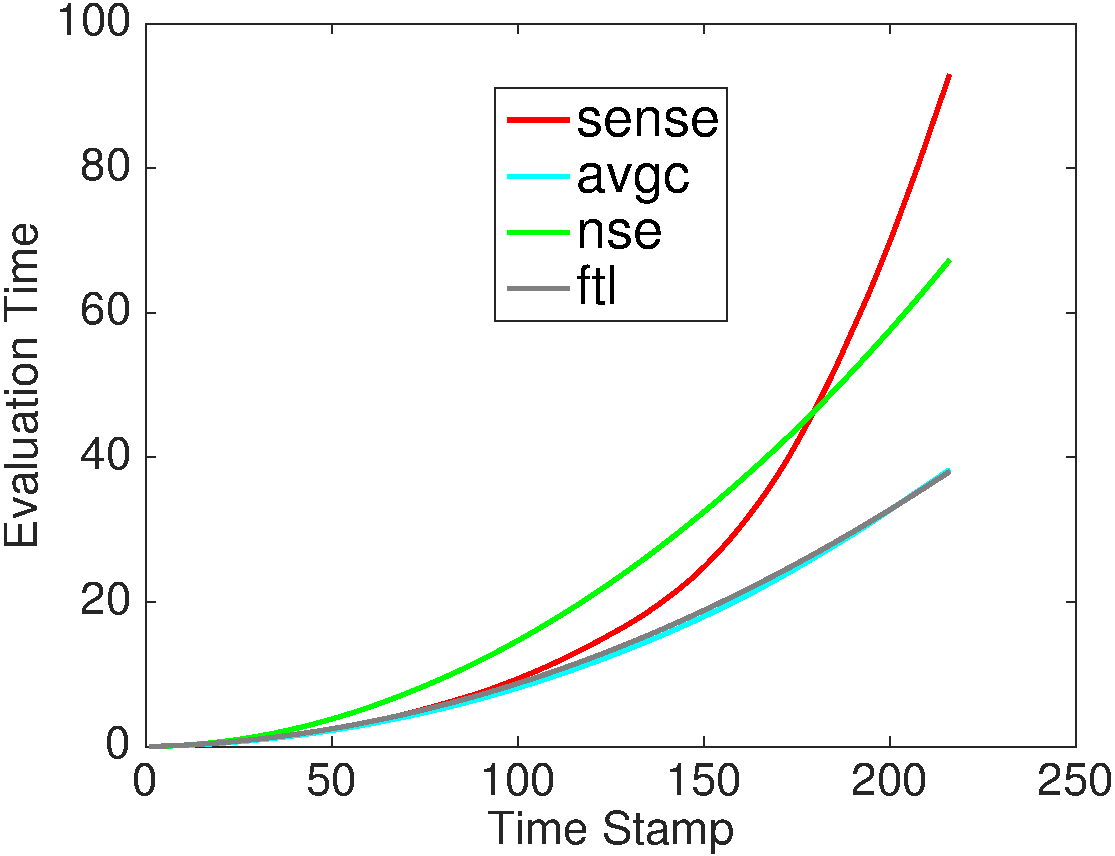
\includegraphics[width=.25\textwidth]{elec2_time.pdf}}
\subfigure[noaa]{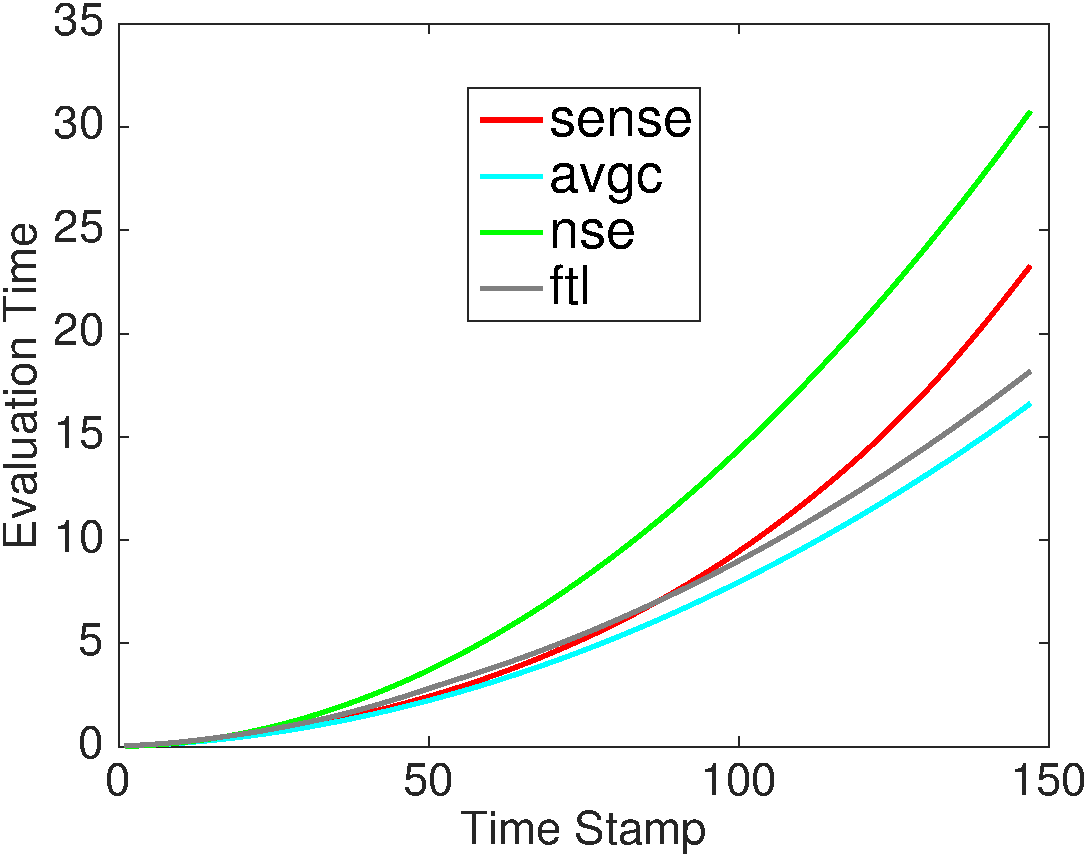
\includegraphics[width=.25\textwidth]{noaa_time.pdf}}
\subfigure[spam]{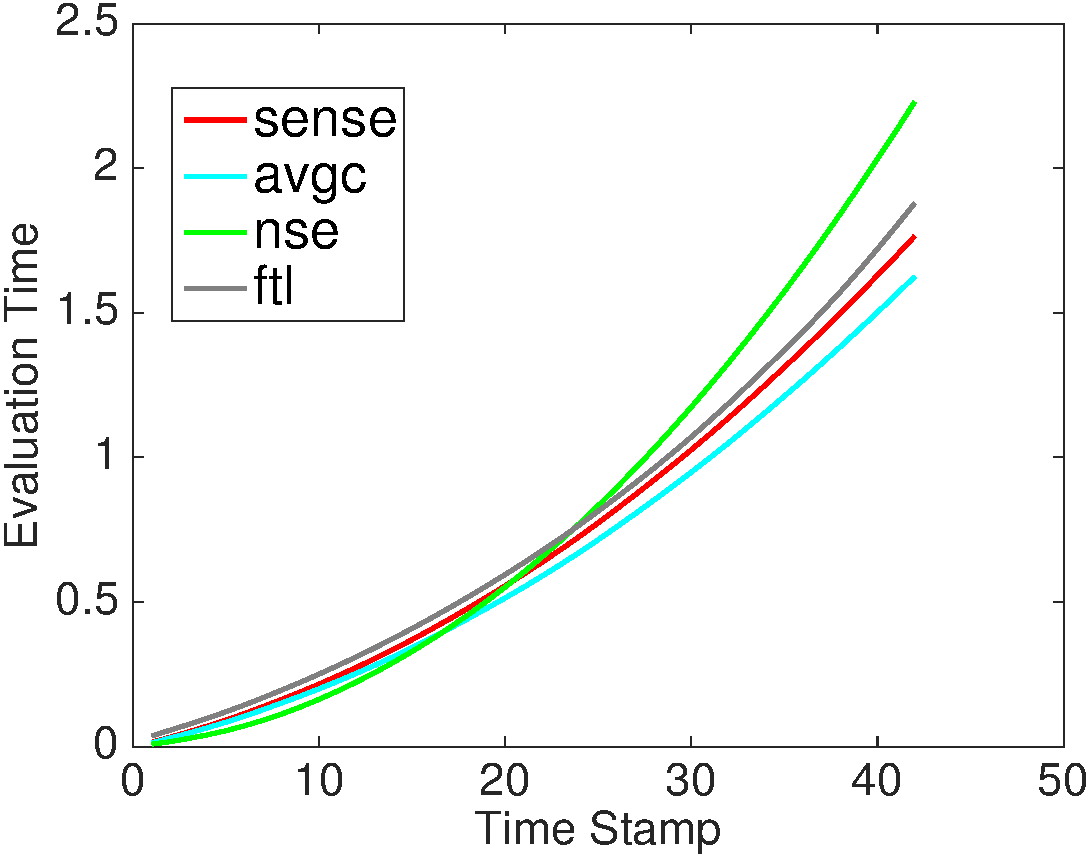
\includegraphics[width=.25\textwidth]{spam_time.pdf}} \\
\subfigure[sea]{\includegraphics[width=.25\textwidth]{sea_time.pdf}}
\subfigure[air]{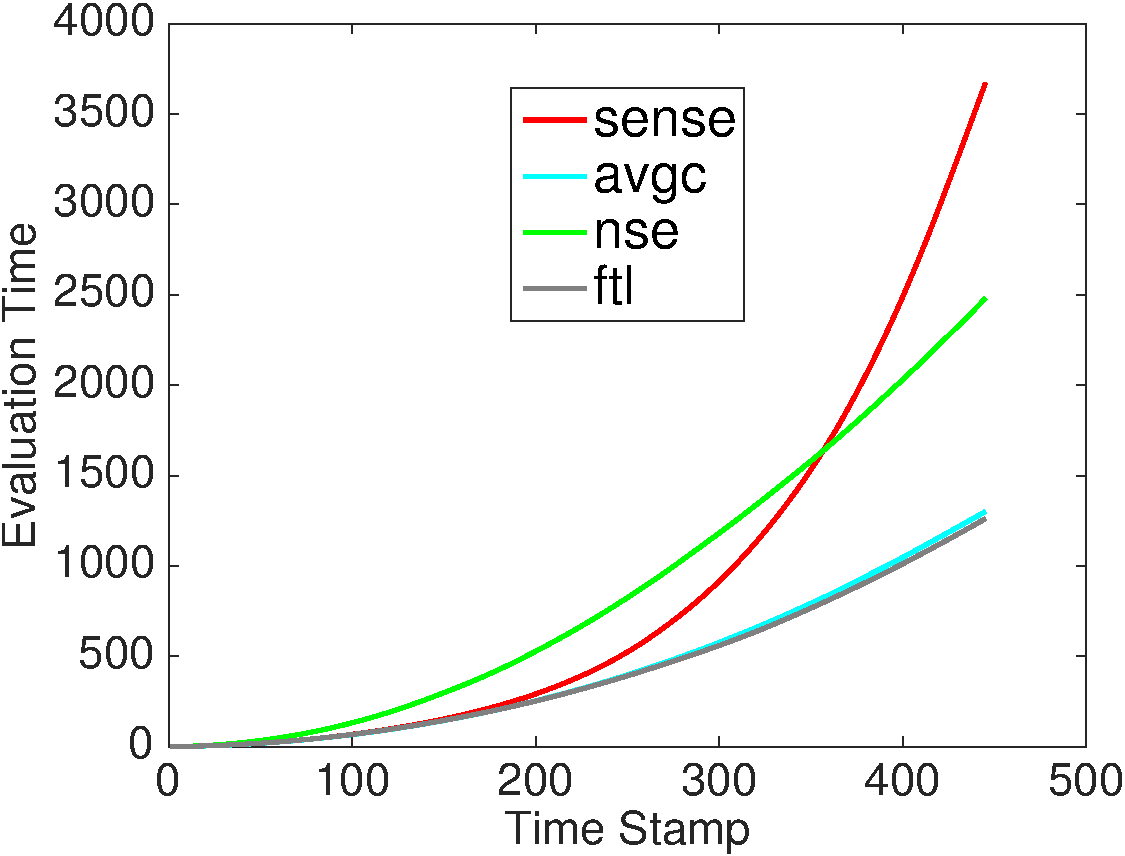
\includegraphics[width=.25\textwidth]{air_time.pdf}\label{fig:times air}}
\subfigure[poker]{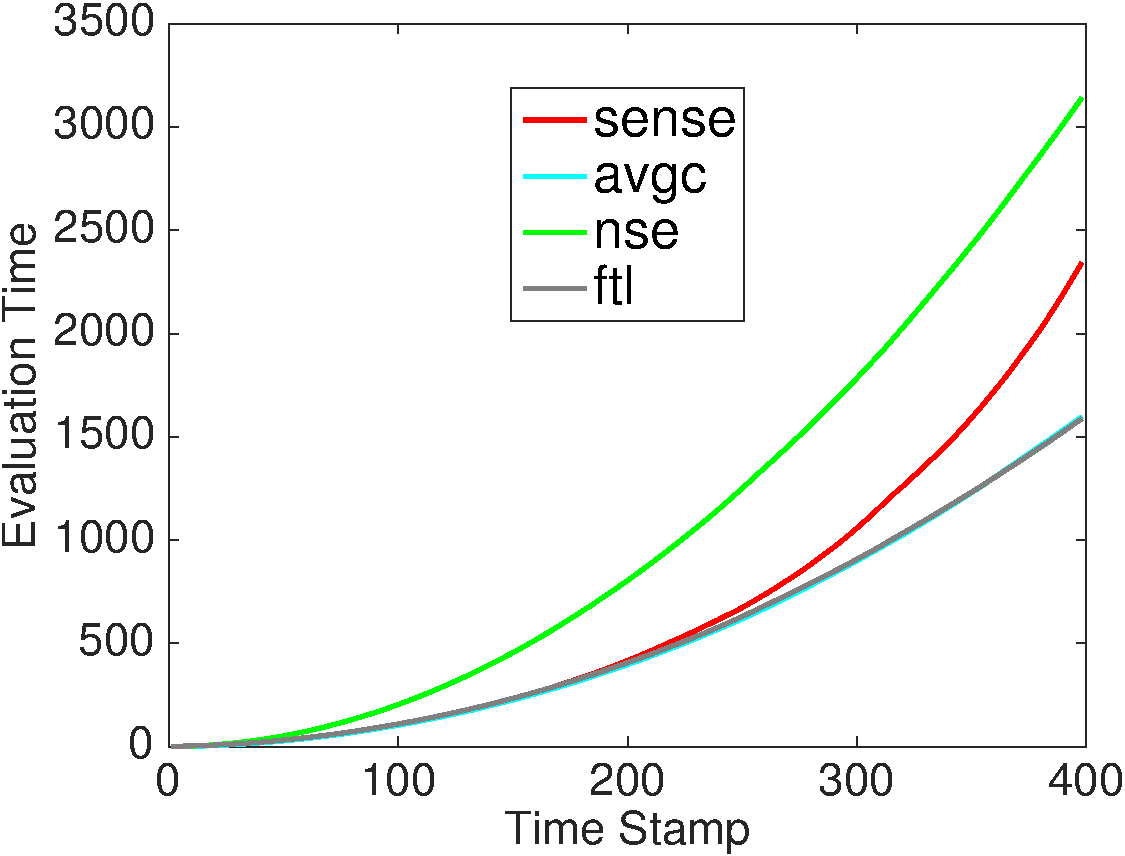
\includegraphics[width=.25\textwidth]{poker_time.pdf}}
\caption{Cumulative evaluation time of the benchmark algorithms. The measurements are represented in seconds. } \label{fig:times}
\end{figure*}

%-------------------------------------------------------------------------
\bibliographystyle{ieeetr}
\bibliography{/Users/gditzler/Dropbox/Public/Research/Bibtex/greg_refs}



\end{document}

